\documentclass{beamer}
\usetheme{Hannover}
\usepackage[utf8]{inputenc}

\title{Aplicación de Algoritmo Genético para Predicción de Alumnos que Aprueban Materias de CB}
\author{Hans Mersch }
\date{Junio 2021}

\begin{document}


\begin{frame}
    \titlepage
\end{frame}

\begin{frame}
    \tableofcontents
\end{frame}

\section{Introducción}
\begin{frame}
    \frametitle{Por que es necesaria realizar esta predicción?}
    \pause
    \begin{columns}
    \column{0.5\textwidth}
    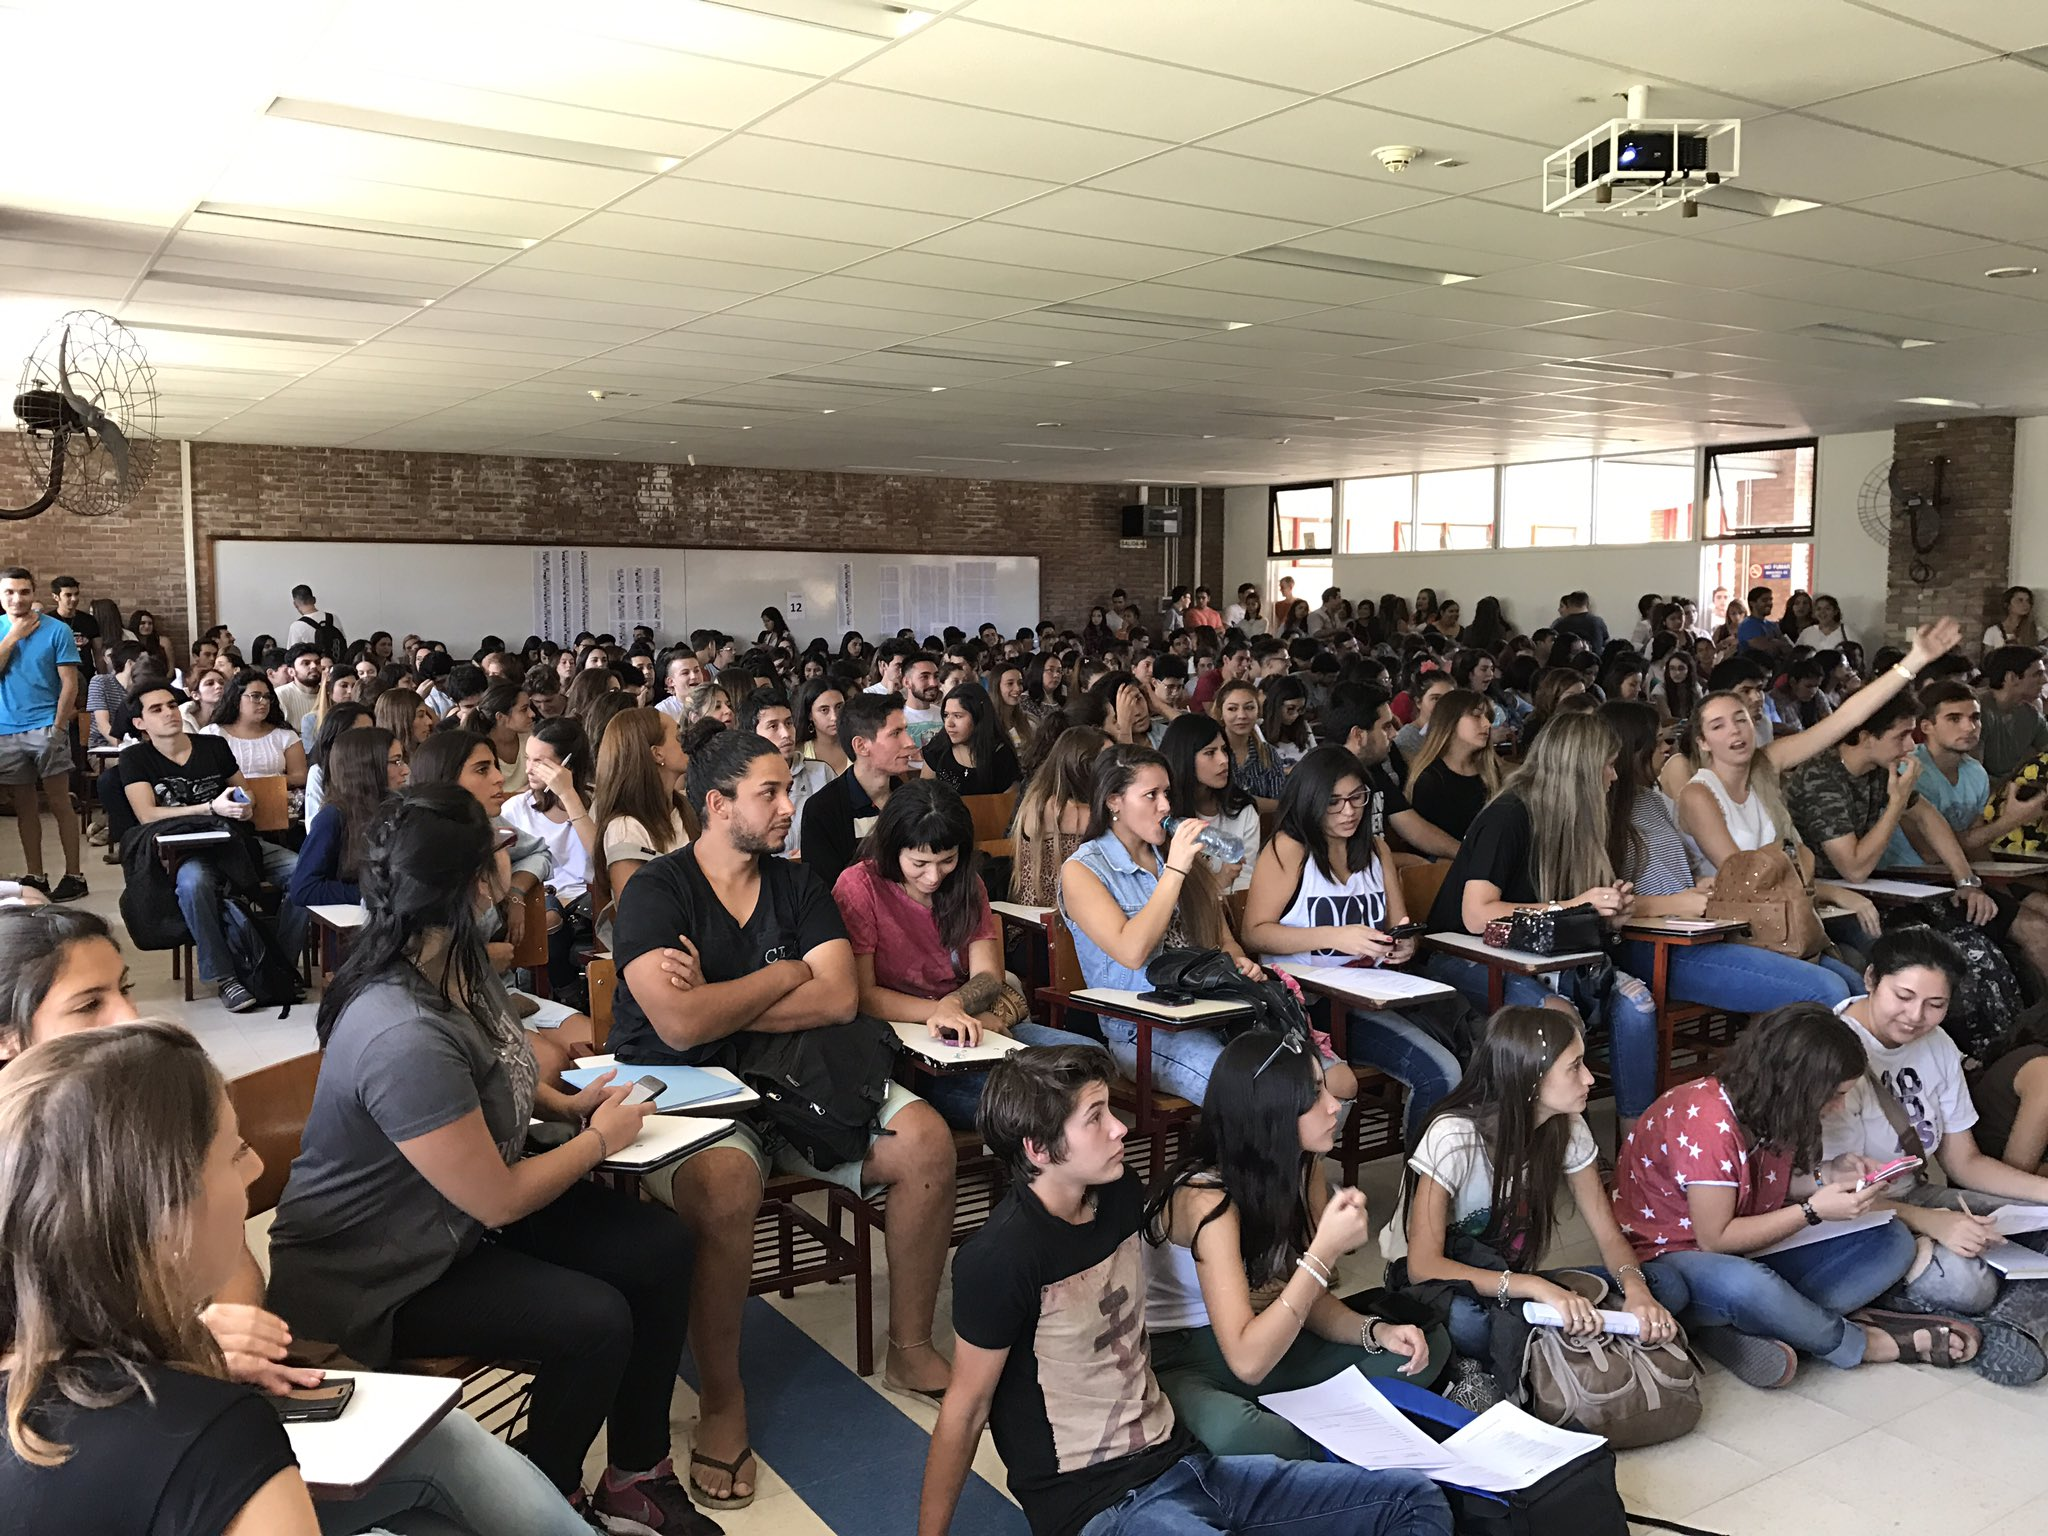
\includegraphics[width=\columnwidth]{Imagenes/C_llena.jpg}
    Sección completamente llena
    \pause
    \column{0.5\textwidth}
    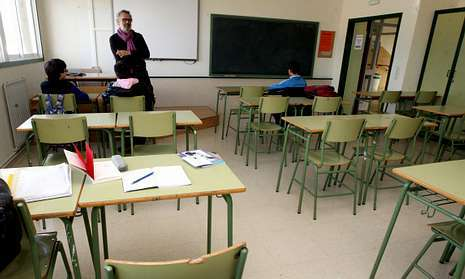
\includegraphics[width=\columnwidth]{Imagenes/C_vacia.jpg}
    Sección con pocos alumnos inscritos
    \end{columns}
\end{frame}

\section{Resultados del primer parcial}
\begin{frame}
    \frametitle{Redes Neuronales}
    \begin{figure}
        \centering
        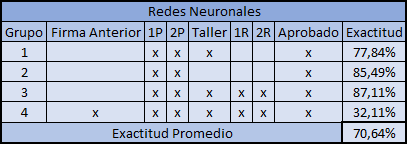
\includegraphics[width=0.7\textwidth]{Imagenes/Resultado_RN.png}

    \end{figure}
\end{frame}

\begin{frame}
    \frametitle{Regresión Logística}
    \begin{figure}
        \centering
        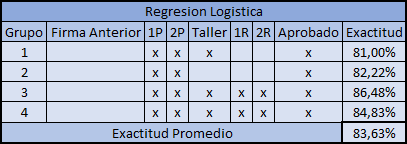
\includegraphics[width=0.7\textwidth]{Imagenes/Resultado_RL.png}
    \end{figure}
\end{frame}

\begin{frame}{Comparación de Modelos}
    \begin{columns}
    \column{0.7\textwidth}
    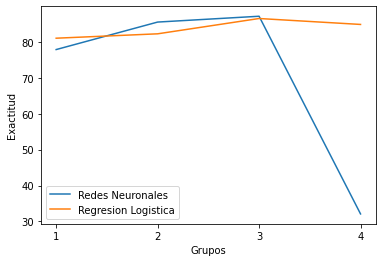
\includegraphics[width=\columnwidth]{Imagenes/Comparacion.png}
    
    \column{0.3\textwidth}
    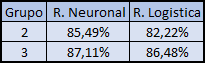
\includegraphics[width=\columnwidth]{Imagenes/Comparacion_2.png}
    
    \end{columns}
\end{frame}

\section{Selección del Algoritmo a Utilizar}

\begin{frame}{Algoritmo de Fuerza Bruta}
    Dado un conjunto de parámetros iniciales, este algoritmo prueba todas las combinaciones posibles hasta encontrar la mejor combinación posible de estos parámetros.
    \begin{figure}
        \centering
        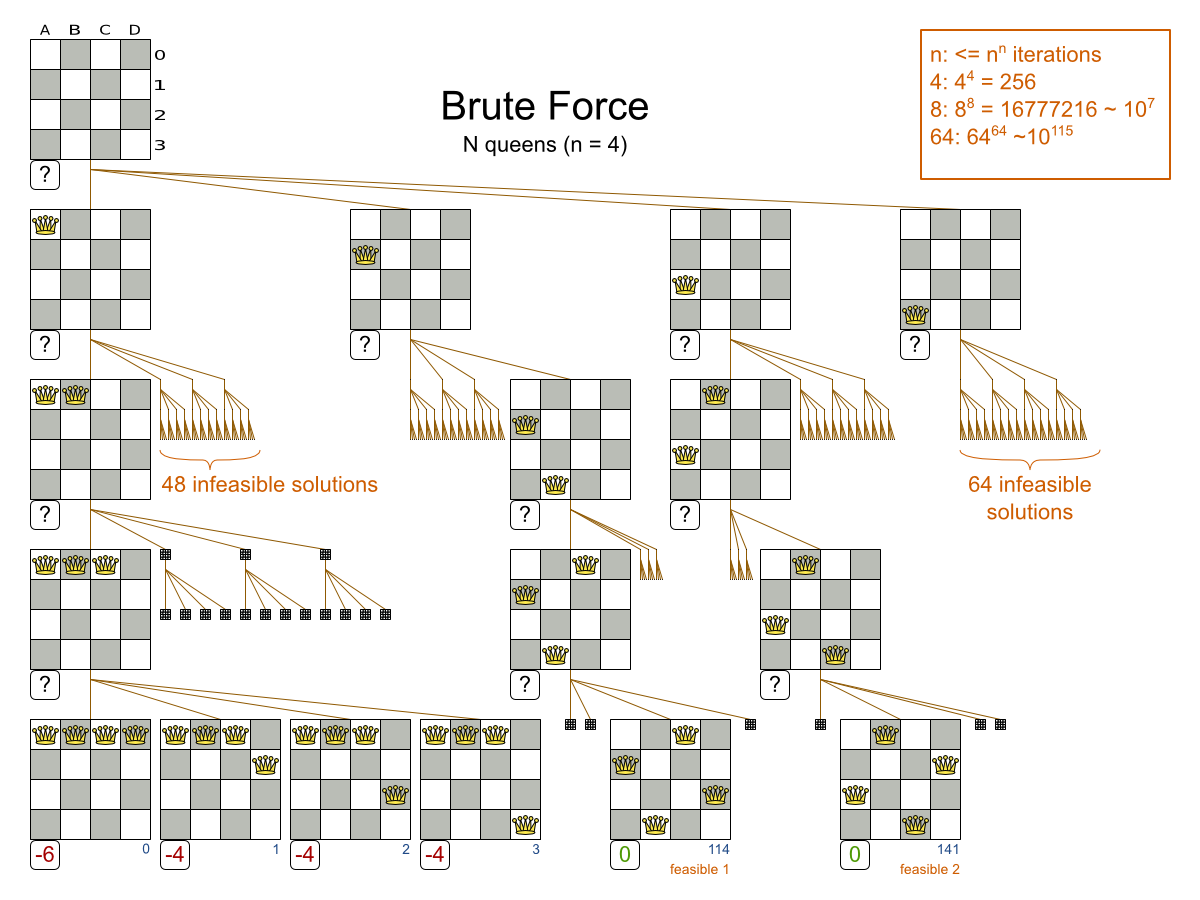
\includegraphics[width=0.7\textwidth]{Imagenes/n_reinas.png}
    \end{figure}
\end{frame}

\begin{frame}
    \frametitle{Algoritmo Genético}
    El algoritmo genético es una búsqueda heurística que está inspirada en la teoría natural de la evolución de Darwin. Este algoritmo refleja el proceso de selección natural, donde los individuos más aptos son seleccionados para reproducirse en orden, para producir descendencia de la siguiente generación.
    
    \begin{figure}
        \centering
        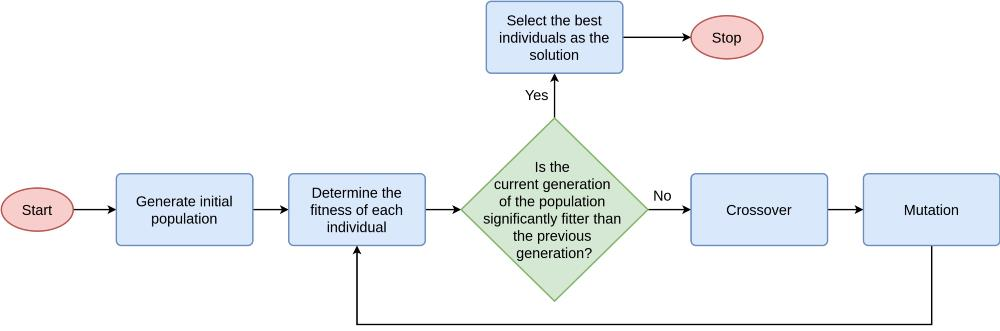
\includegraphics[width=0.7\textwidth]{Imagenes/AG_flowchart.jpg}
    \end{figure}
\end{frame}


\begin{frame}{DeepEvolve}
    \begin{columns}
    \column{0.3\textwidth}
    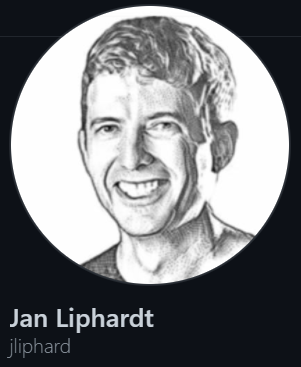
\includegraphics[width=0.8\columnwidth]{Imagenes/jan.png}
    \begin{itemize}
        \item Profesor de Bioingeniería de la Universidad de Stanford
        \item Jefe en Tecnología en Enya.ai
    \end{itemize}
    
    \column{0.7\textwidth}
    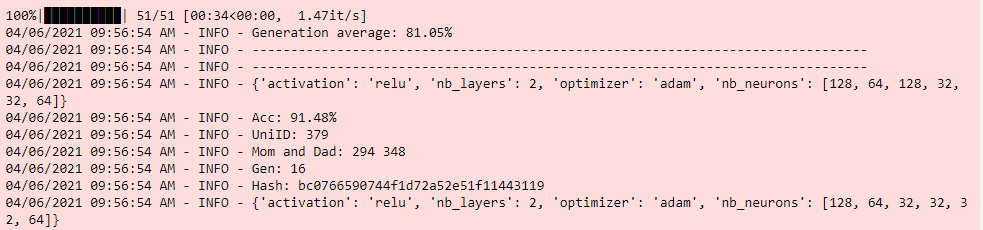
\includegraphics[width=\columnwidth]{Imagenes/algoritmo.png}
    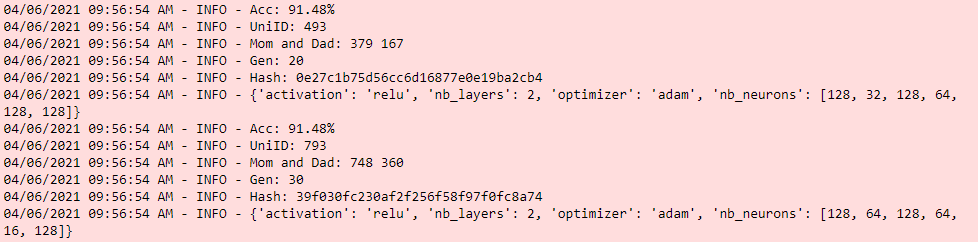
\includegraphics[width=\columnwidth]{Imagenes/algoritmo2.png}
    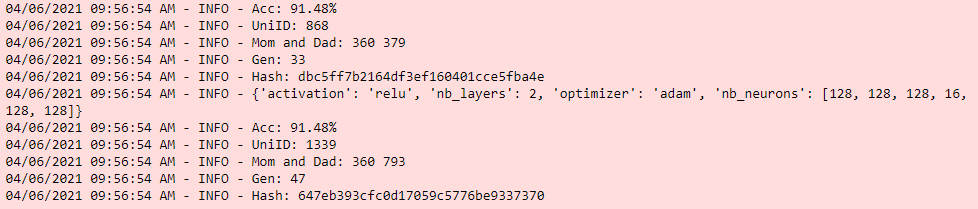
\includegraphics[width=\columnwidth]{Imagenes/algoritmo3.png}
    \end{columns}
\end{frame}

\section{Modelos a Implementar}
\begin{frame}{Modelos a Implementar}
    \begin{figure}
        \centering
        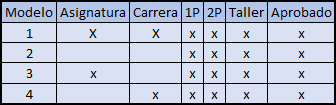
\includegraphics[width=0.7\textwidth]{Imagenes/modelos.png}
    \end{figure}
\end{frame}

\section{Resultados}

\begin{frame}{Resultados de la Implementación}
    \begin{figure}
        \centering
        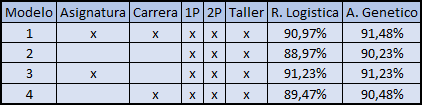
\includegraphics[width=0.7\textwidth]{Imagenes/modelos2.png}
    \end{figure}
\end{frame}

\section{Mejoras para la Siguiente Etapa}
\begin{frame}{Early Stop}
    \begin{columns}
    \column{0.45\textwidth}
    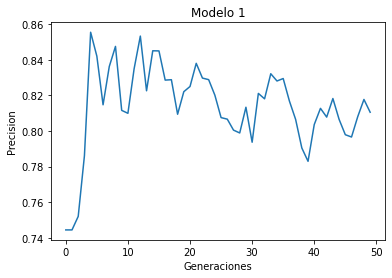
\includegraphics[width=\columnwidth]{Imagenes/AG1.png}
    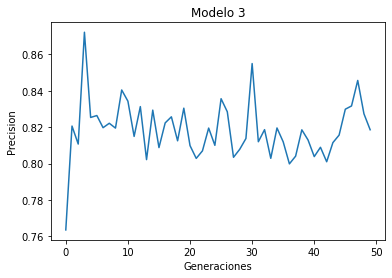
\includegraphics[width=\columnwidth]{Imagenes/AG3.png}
    
    \column{0.45\textwidth}
    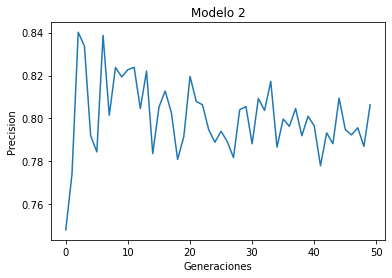
\includegraphics[width=\columnwidth]{Imagenes/AG2.png}
    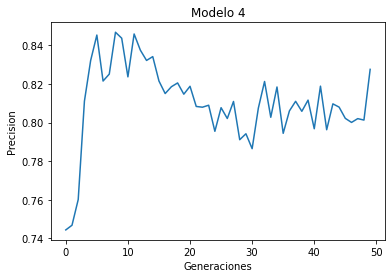
\includegraphics[width=\columnwidth]{Imagenes/AG4.png}
    
    \end{columns}
\end{frame}

\begin{frame}
    Muchas Gracias!
\end{frame}

\end{document}
